\section{Referencia de la Clase Articulo}
\label{classArticulo}\index{Articulo@{Articulo}}
Clase art\'{\i}culo.  


{\tt \#include $<$articulo.h$>$}

Diagrama de herencias de Articulo\begin{figure}[H]
\begin{center}
\leavevmode
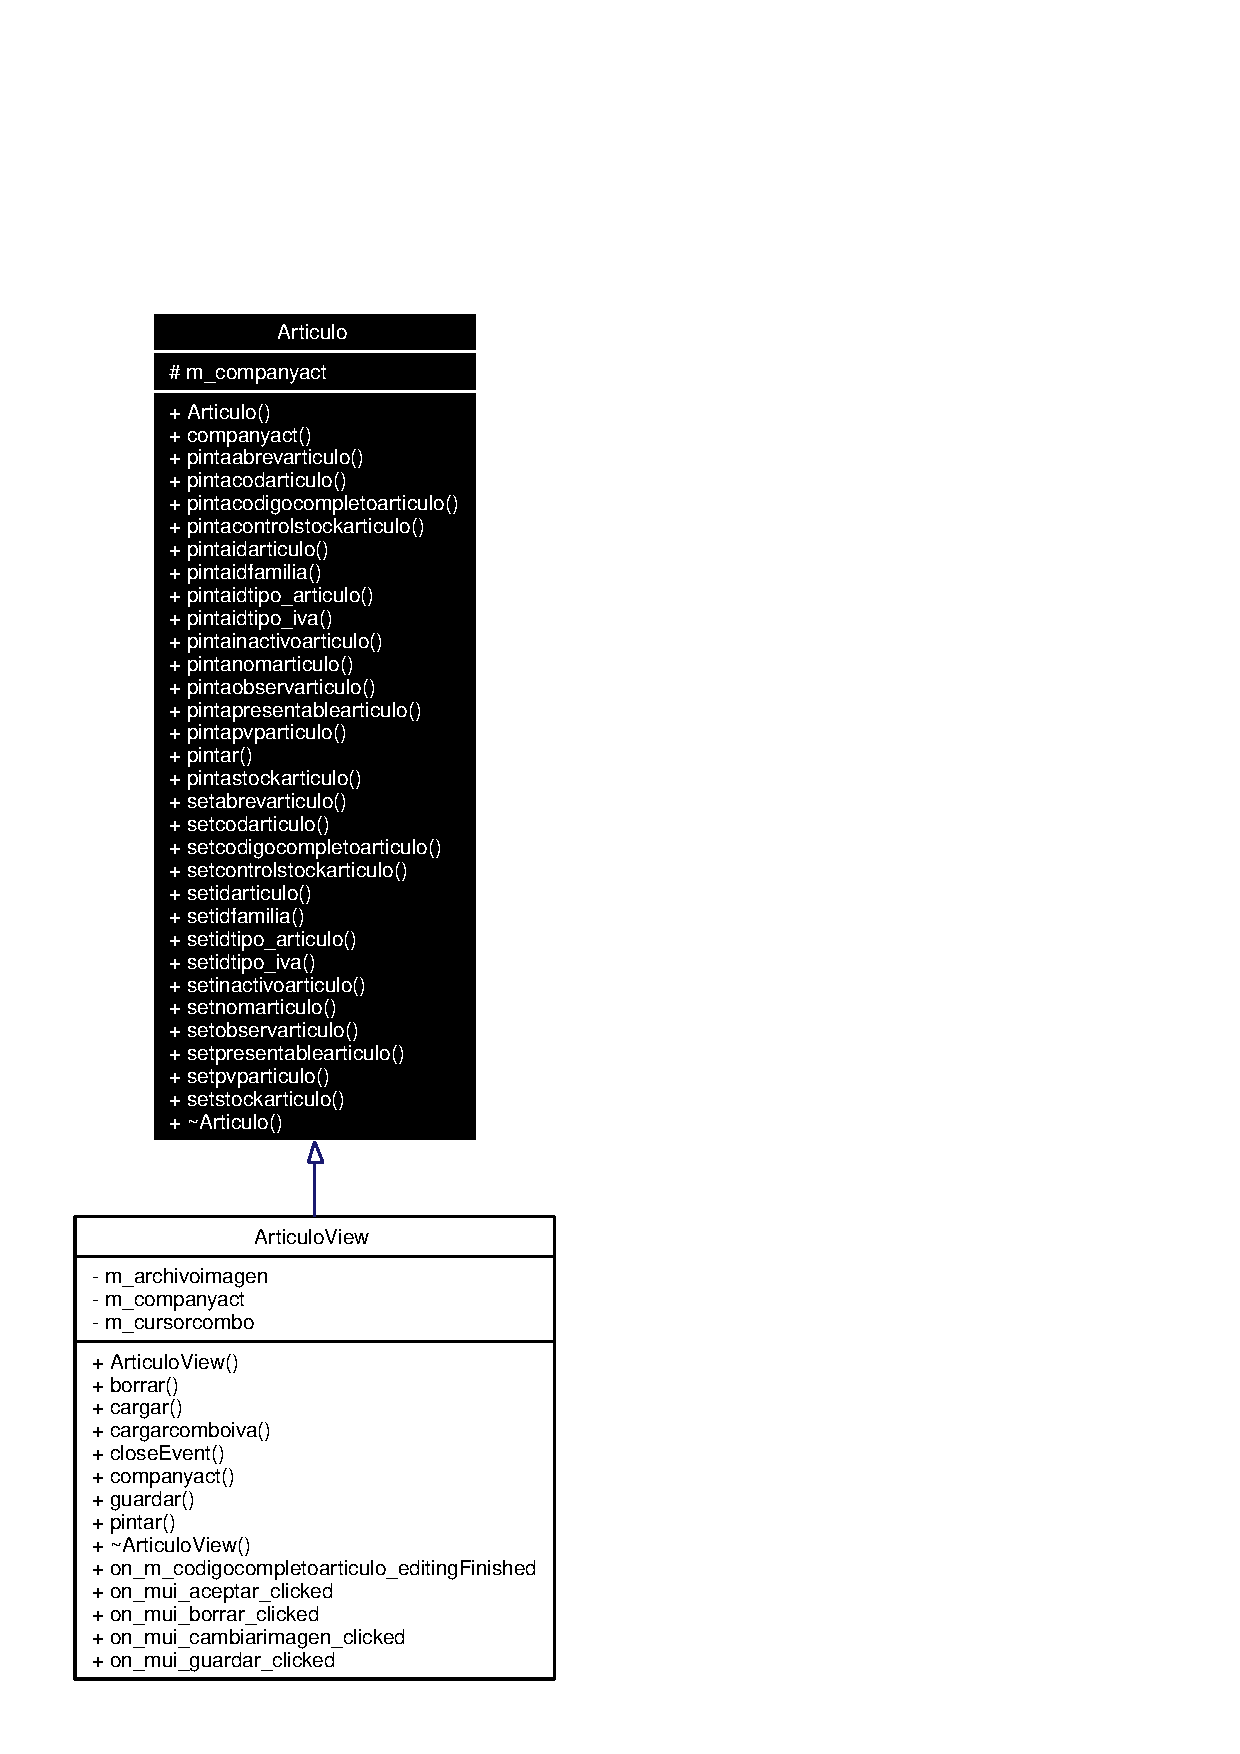
\includegraphics[width=133pt]{classArticulo__inherit__graph}
\end{center}
\end{figure}
Diagrama de colaboraci\'{o}n para Articulo:\begin{figure}[H]
\begin{center}
\leavevmode
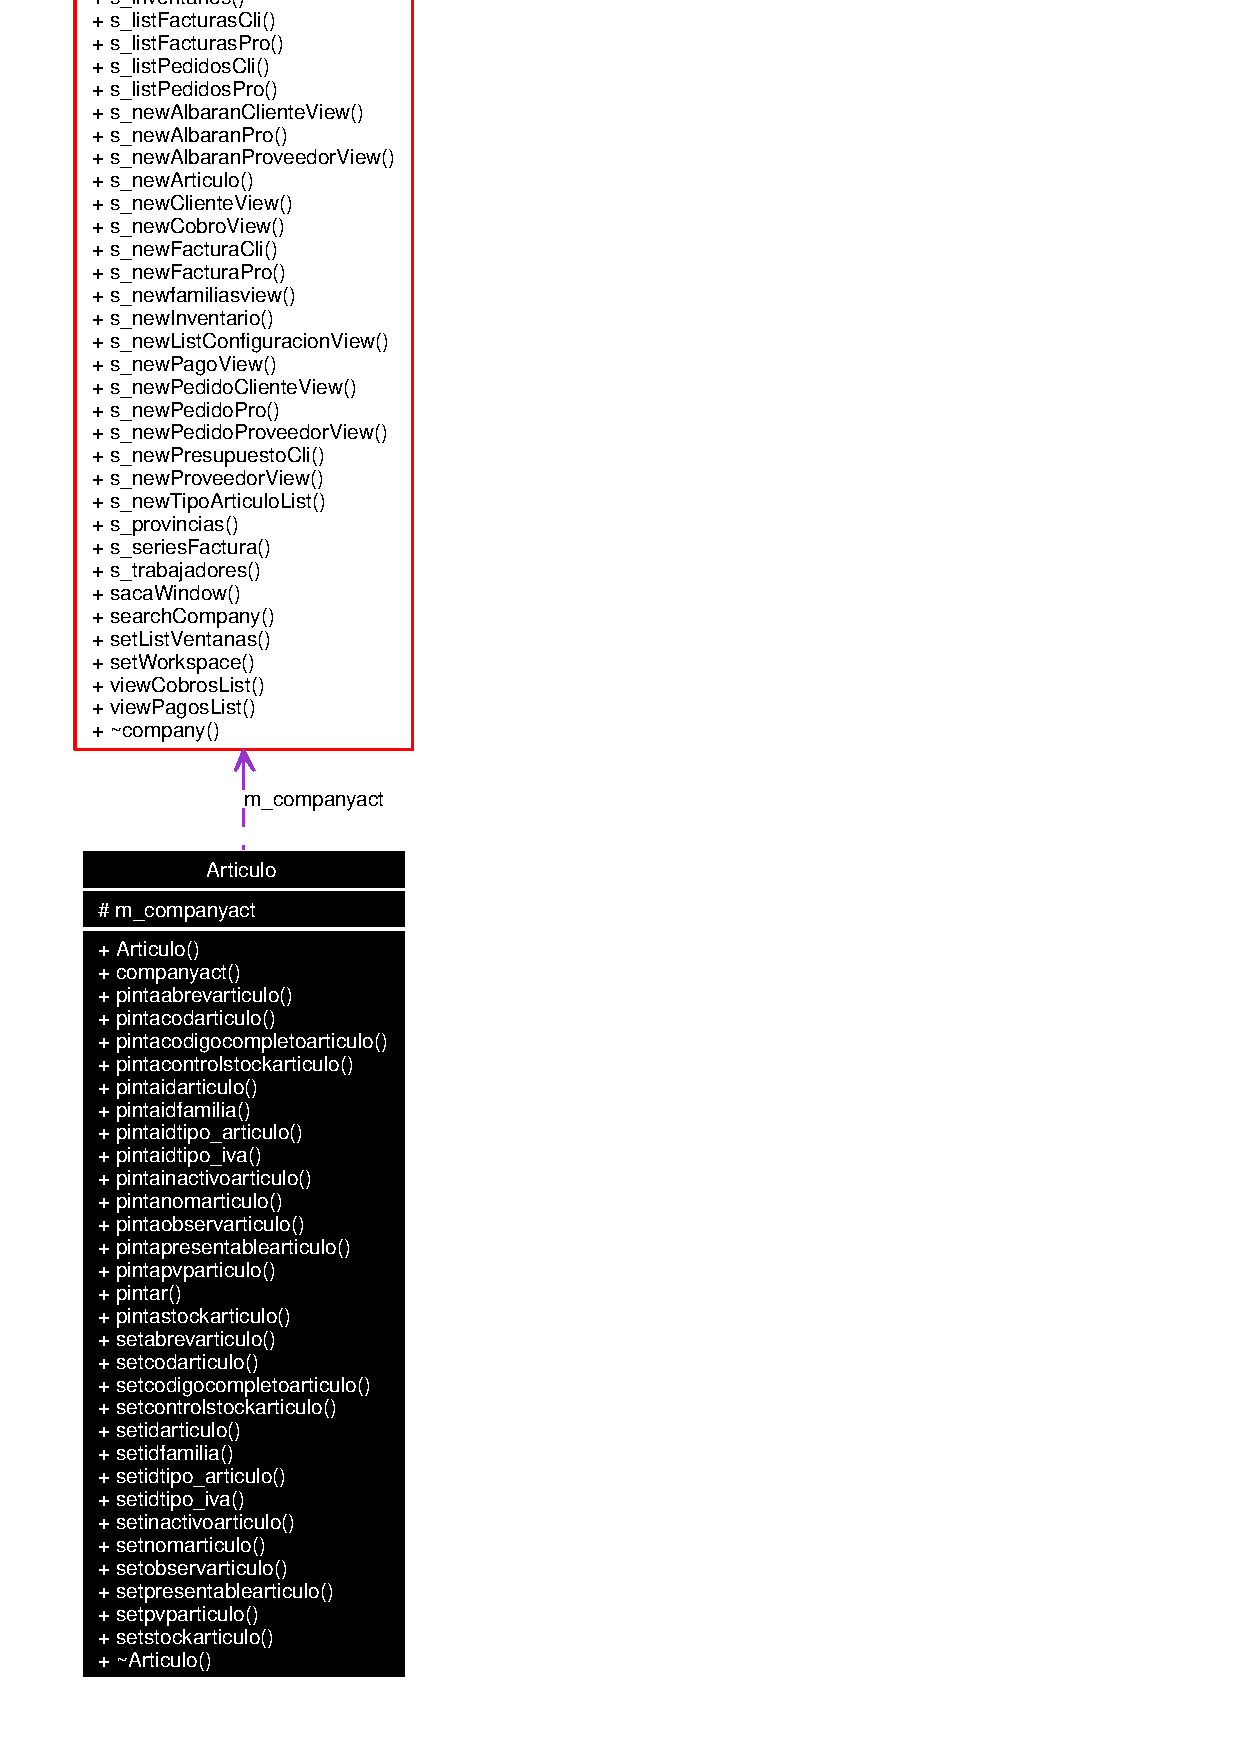
\includegraphics[width=99pt]{classArticulo__coll__graph}
\end{center}
\end{figure}
\subsection*{M\'{e}todos p\'{u}blicos}
\begin{CompactItemize}
\item 
{\bf Articulo} ({\bf company} $\ast$)\label{classArticulo_a0}

\item 
{\bf company} $\ast$ {\bf companyact} ()\label{classArticulo_a1}

\item 
virtual void {\bf pintaabrevarticulo} (QString)\label{classArticulo_a2}

\item 
virtual void {\bf pintacodarticulo} (QString)\label{classArticulo_a3}

\item 
virtual void {\bf pintacodigocompletoarticulo} (QString)\label{classArticulo_a4}

\item 
virtual void {\bf pintacontrolstockarticulo} (QString)\label{classArticulo_a5}

\item 
virtual void {\bf pintaidarticulo} (QString)\label{classArticulo_a6}

\item 
virtual void {\bf pintaidfamilia} (QString)\label{classArticulo_a7}

\item 
virtual void {\bf pintaidtipo\_\-articulo} (QString)\label{classArticulo_a8}

\item 
virtual void {\bf pintaidtipo\_\-iva} (QString)\label{classArticulo_a9}

\item 
virtual void {\bf pintainactivoarticulo} (QString)\label{classArticulo_a10}

\item 
virtual void {\bf pintanomarticulo} (QString)\label{classArticulo_a11}

\item 
virtual void {\bf pintaobservarticulo} (QString)\label{classArticulo_a12}

\item 
virtual void {\bf pintapresentablearticulo} (QString)\label{classArticulo_a13}

\item 
virtual void {\bf pintapvparticulo} (QString)\label{classArticulo_a14}

\item 
virtual void {\bf pintar} ()
\item 
virtual void {\bf pintastockarticulo} (QString)\label{classArticulo_a16}

\item 
void {\bf setabrevarticulo} (QString val)\label{classArticulo_a17}

\item 
void {\bf setcodarticulo} (QString val)\label{classArticulo_a18}

\item 
void {\bf setcodigocompletoarticulo} (QString val)\label{classArticulo_a19}

\item 
void {\bf setcontrolstockarticulo} (QString val)\label{classArticulo_a20}

\item 
void {\bf setidarticulo} (QString val)\label{classArticulo_a21}

\item 
void {\bf setidfamilia} (QString val)\label{classArticulo_a22}

\item 
void {\bf setidtipo\_\-articulo} (QString val)\label{classArticulo_a23}

\item 
void {\bf setidtipo\_\-iva} (QString val)\label{classArticulo_a24}

\item 
void {\bf setinactivoarticulo} (QString val)\label{classArticulo_a25}

\item 
void {\bf setnomarticulo} (QString val)\label{classArticulo_a26}

\item 
void {\bf setobservarticulo} (QString val)\label{classArticulo_a27}

\item 
void {\bf setpresentablearticulo} (QString val)\label{classArticulo_a28}

\item 
void {\bf setpvparticulo} (QString val)\label{classArticulo_a29}

\item 
void {\bf setstockarticulo} (QString val)\label{classArticulo_a30}

\end{CompactItemize}
\subsection*{Atributos protegidos}
\begin{CompactItemize}
\item 
{\bf company} $\ast$ {\bf m\_\-companyact}\label{classArticulo_p0}

\end{CompactItemize}


\subsection{Descripci\'{o}n detallada}
Clase art\'{\i}culo. 



\subsection{Documentaci\'{o}n de las funciones miembro}
\index{Articulo@{Articulo}!pintar@{pintar}}
\index{pintar@{pintar}!Articulo@{Articulo}}
\subsubsection{\setlength{\rightskip}{0pt plus 5cm}void Articulo::pintar ()\hspace{0.3cm}{\tt  [virtual]}}\label{classArticulo_a15}


Disparamos los plugins con presupuesto\_\-imprimir\-Presupuesto. 

Reimplementado en {\bf Articulo\-View} {\rm (p.\,\pageref{classArticuloView_a7})}.

La documentaci\'{o}n para esta clase fu\'{e} generada a partir de los siguientes archivos:\begin{CompactItemize}
\item 
articulo.h\item 
articulo.cpp\end{CompactItemize}
